\documentclass[oneside,12pt]{Classes/aesm_edspia}

\usepackage{minitoc}
\usepackage[latin1]{inputenc}
\usepackage[english,french]{babel}
\usepackage[T1]{fontenc}
\usepackage{amsmath}
\usepackage{lmodern}%font modern
\rmfamily
\DeclareFontShape{T1}{lmr}{bx}{sc}{<->ssub * cmr/bx/sc}{}
\usepackage{lettrine}
\usepackage{tabularx}
\usepackage{epsfig, floatflt, amssymb}
\usepackage{moreverb} %% pour le verbatim en boite
\usepackage{cases}%equations en systemes numerotes - soluce possible package : CASES
\usepackage{multirow} %% pour regrouper un texte sur plusieurs lignes dans une table
\usepackage{url} %% pour citer les url par \url
\usepackage[all]{xy} %% pour la barre au dessus des symboles
\usepackage{textcomp} %% pour le symbol pour mille par \textperthousand et degres par \degres
\usepackage[right]{eurosym}
\usepackage{setspace} %interligne simple, double etc...
\usepackage{Classes/eurosans} %%pour le symbole \euro
\usepackage{epic,eepic}
\usepackage{soul}
\usepackage[nottoc]{tocbibind} % tables des figures, des matieres et autres dans la TOC
\usepackage{fancybox}
\usepackage[leftcaption]{sidecap}
\usepackage[labelsep=endash, textfont={footnotesize, singlespacing}, margin=10pt, format=plain, labelfont=bf]{caption}
\usepackage[Conny]{Classes/fncychap} %en tete chapitrage
\newcommand{\ie}{c.-\`a-d.~}
\hbadness=10000% pb d'overfull box regle
\hfuzz=50pt
\pdfcompresslevel9 % pour compresser le pdf final au maximum
\pdfoptionpdfminorversion=5 % pour accepte les images PDF version 1.5 (ex: celles produites par Office 2007)
\def\underscore{\char`\_}
\makeatletter
\renewcommand{\thesection}{\arabic {section}}
\renewcommand{\SC@figure@vpos}{c}% centrer verticalement le caption avec le package sidecap...
\renewcommand{\fnum@figure}{\small\textbf{Figure~\thefigure}}
\renewcommand{\fnum@table}{\small\textbf{Tableau~\thetable}}

\makeatother
\usepackage{subfig}
\def\thechapter{\Roman{chapter}}

%\usepackage[framed,numbered,autolinebreaks,useliterate]{Classes/mcode}


%%% Listings

\usepackage{listings}
\lstloadlanguages{xml, java}

	 \usepackage{listings}
  \usepackage{courier}
 \lstset{
         basicstyle=\footnotesize\ttfamily,
         %numbers=left,
         numberstyle=\tiny,
         %stepnumber=2,
         numbersep=5pt,
         tabsize=2,
         extendedchars=true,
         breaklines=true,
         keywordstyle=\color[rgb]{0.43,0,0}\textbf,
    		frame=b,
         commentstyle=\color[rgb]{0.51,0.51,0.51} \textit ,
         stringstyle=\ttfamily  \color[rgb]{0,0.44,0} ,
         showspaces=false,
         showtabs=false,
         xleftmargin=17pt,
         framexleftmargin=17pt,
         framexrightmargin=5pt,
         framexbottommargin=4pt,
         %backgroundcolor=\color{lightgray},
         showstringspaces=false
 }

 \usepackage{caption}
\DeclareCaptionFont{white}{\color{white}}
\DeclareCaptionFont{red}{\color{red}}
\DeclareCaptionFont{black}{\color{black}}
\DeclareCaptionFormat{listing}{\colorbox[cmyk]{0.43, 0.35, 0.35,0.01}{\parbox{\textwidth}{\hspace{15pt}#1#2#3}}}
\captionsetup[lstlisting]{format=listing,labelfont=black,textfont=white, singlelinecheck=false, margin=0pt, font={bf,footnotesize}}


%%%%%%%%%%%%%%%%%%%%%%%%%%%%%%%%%%%%%%%%%%%
\begin{document}
%%%%%%%%%%%%%%%%%%%%%%%%%%%%%%%%%%%%%%%%%%%
\renewcommand\figurename{\small\textbf{Figure}}

\addtocounter{page}{-1}%pour revenir e 0

% Pour remplir la page de garde
\AuteurA{Marouane} {ELKAMEL}
%\AuteurB{Flen2} {FOULENI}
%\AuteurC{Flen3} {FOULENI}
%\AuteurD{Flen4} {FOULENI}
\Encadrant{Mr}{Aymen}{SELLAOUTI}
\EncadrantS{Mr} {Anis} {KALLEL}

\Filiere{GL}
\datesout{--/--/2019}



\President{M. President} {FLEN}     %% President du Jury
\RapporteurA{Mme. Rapporteur} {FLENA} %%Rapporteur



\AnneeUniv{2018/2019}

%%%%%%%%%%%%%%%%%%%%%%%%%%%%%%%%%%%%%%%%%%%
\makethese %% cree la couverture.

\onehalfspacing

% une page blanche (deuxieme de couverture)
\newpage\thispagestyle{empty}\addtocounter{page}{-3}
\null\newpage\thispagestyle{empty}


\frontmatter %numerotation en iii
\pagestyle{fancy}
\fancyhf{}
\fancyhead[R]{Remerciements}
\fancyfoot[R]{\thepage}
\renewcommand{\headrulewidth}{0.5pt}
\renewcommand{\footrulewidth}{0pt}

\chapter*{Dedication}
%===================================================================

Thanks\dots
\chapter*{Acknowledgments}

This work would not have been possible without the valuable cooperation of a number of people I would like to pay tribute to.\newline

I would like to thank all those who have made this internship a rewarding and enjoyable experience, especially :\newline

\textbf{Mr. Nebras JEMEL}, co-founder and CEO of Flouci, for believing in me from day one, my internship tutor \textbf{Mr. Anis KALLEL}, co-founder and CTO, who introduced me to the team and helped me greatly throughout my journey. Thank you for your advice and guidance throughout this internship. \newline

The \textbf{"Flouci"} team, my second family, for their support and direction. More importantly, their devotion and passion for what we are doing inspires me every day.\newline

I would especially like to thank my supervisor \textbf{Mr. Aymen SELLOAUTI} for his availability, remarks, and advice. I also would like to express my respect and my gratitude to him.\newline

Finally, I also express my sincere appreciation to the members of the jury : \textbf{Mr Flen} and \textbf{Mr Flen} for accepting to evaluate my work.


%%%%%%%% TOC

%profondeur dans la table des matieres et de la numerotation des sections

\setcounter{secnumdepth}{3}
\setcounter{tocdepth}{3}


\renewcommand{\contentsname}%
    {Table des Matieres}%

%%%%minitoc
\dominitoc % genere la minitoc
\nomtcrule % supprime les lignes horizontales de la minitoc
\renewcommand{\mtctitle}{Plan} % Modifie le titre de la minitoc

%%%%
\tableofcontents

\renewcommand{\headrulewidth}{0.5pt}
\renewcommand{\footrulewidth}{0pt}
\fancyhead[R]{Table des Matieres}


%%%%%%%% Figures

\makeatletter
%\renewcommand{a\thefigure}{\@arabic\c@figure}
\@addtoreset{figure}{chapter}
\makeatother

\renewcommand{\headrulewidth}{0.5pt}
\renewcommand{\footrulewidth}{0pt}
\renewcommand\listfigurename{Liste des Figures}
\listoffigures \mtcaddchapter

\fancyhead[R]{Liste des Figures}
\newpage


%%%%%%%% Tableaux

\makeatletter

\renewcommand{\headrulewidth}{0.5pt}
\renewcommand{\footrulewidth}{0pt}
\renewcommand\listtablename{Liste des Tableaux}

\listoftables  \mtcaddchapter

\fancyhead[R]{Liste des Tableaux}

%%%%%%%%%%%%%%%%%%%%%%%%%%%%%%%%%%%
%\fancyhead[R]{Resumes}

\chapter*{Summary}
\addcontentsline{toc}{chapter}{Resume}
%===================================================================

Brief summary \dots

\chapter*{Abstract}
\addcontentsline{toc}{chapter}{Abstract}
%===================================================================

This is the english abstract of your project. It must be longer and presented in more details than the abstract you write on the back of your report.


%%%%%%%%%%%%%%%%%%%%%%%%%%%%%%%%%%%


\mainmatter %numeros arabes
\pagestyle{fancy}
\fancyhead[R]{Introduction Generale}
\chapter*{General Introduction}
\graphicspath{{Introduction/figures/}}
\addcontentsline{toc}{chapter}{General Introduction}
\begin{spacing}{1.2}
%==================================================================================================%

In the modern software world APIs are becoming a must for every tech company to allow products to be integrated by developers in multiple Apps.

APIs do all this by "exposing" some of a product's internal functions to the outside world in a limited fashion. That makes it possible for applications to share data and take actions on one another's behalf without requiring developers to share all of their software's code. 



\begin{figure}[!ht]\centering
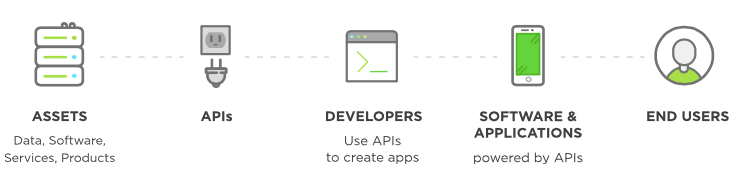
\includegraphics[scale=0.6]{API.png}
\caption{APIs }
\label{fig:fig1}
\end{figure}

That's the reason why KAOUN, a Tunisian FinTech start-up, decided to create its own developers API for its main product FLOUCI which is a mobile payment solution. This project will expand FLOUCI to the developers world and unleash the full potential of the product, also it could take FLOUCI into new markets and open doors for unlimited integrations.\newline


The following report is a synthesis of the efforts done to build FLOUCI developers API.

 To detail the process of our work, we have divided this report into XX chapters representing the different aspects of our project.

In the first chapter, entitled Project scope, we started with a presentation of the host company. Afterwards, we gave an overview of our project and we detailed the followed methodology for its realization.


The second chapter is about the development disciplines and rules we set during our project development life cycle. It's a detailed explanation of the development practices needed to start our project development in the most efficient way possible. 



We close our work with a general conclusion in which we try to evaluate our contribution as well as we develop our vision for the project's potential improvements.




\end{spacing}

\fancyhf{}
\fancyhead[R]{Introduction Generale}
\fancyfoot[R]{\thepage}
\renewcommand{\headrulewidth}{0.5pt}
\renewcommand{\footrulewidth}{0pt}



\setcounter{mtc}{5} %indique le numero reel du chapitre, pour la mini table des matieres
\chapter{Project Scope}
\minitoc  %insert la minitoc

\graphicspath{{Chapitre1/figures/}}
%==============================================================================
\pagestyle{fancy}
\fancyhf{}
\fancyhead[R]{\bfseries\rightmark}
\fancyfoot[R]{\thepage}
\renewcommand{\headrulewidth}{0.5pt}
\renewcommand{\footrulewidth}{0pt}
\renewcommand{\chaptermark}[1]{\markboth{\MakeUppercase{\chaptername~\thechapter. #1 }}{}}
\renewcommand{\sectionmark}[1]{\markright{\thechapter.\thesection~ #1}}

\begin{spacing}{1.2}
%==============================================================================

\section*{Introduction}
\section{Host company presentation} 
\subsection{Presentation of Kaoun}
\subsection{Presentation of Flouci}
\section{Project overview}
\subsection{Project Context}
\subsection{Study of the existing}
\subsection{Project goals}
\section{Methodology}
\subsection{Agile methodology}
\subsection{SCRUM methodology}
\subsection{Lean software development}
\section*{Conclusion}


Une etude theorique \cite{YOUSFI2015} peut contenir l'une et/ou l'autre de ces deux parties :
Elle est en general realisee quand on va developper un module supplementaire sur un 
logiciel existant, ou si on va modifier une application existante. L'etude de l'existant
consiste e expliquer ce qui existe deje dans votre environnement de travail.


La conclusion est en general sans numerotation, et n'apparaet pas dans la table des matieres.

C'est une etude assez detaillee sur ce qui existe sur le marche ou dans la litterature (d'oe 
le terme etat de l'art), qui permet de repondre e la problematique. L'idee ici est de faire 
un comparatif entre les solutions existantes, mais surtout d'analyser le resultat de cette 
comparaison et de dire pourquoi ne sont-elles pas satisfaisantes pour repondre e votre 
problematique.
\begin{figure}[!ht]\centering

\includegraphics[scale=0.9]{art.jpg}
\caption{state of the art}
\label{fig:fig1}
\end{figure}





%==============================================================================
\end{spacing}


\setcounter{chapter}{1}
\chapter{Conception}
\minitoc %insert la minitoc
\graphicspath{{Chapitre2/figures/}}

%\DoPToC

%==============================================================================
\pagestyle{fancy}
\fancyhf{}
\fancyhead[R]{\bfseries\rightmark}
\fancyfoot[R]{\thepage}
\renewcommand{\headrulewidth}{0.5pt}
\renewcommand{\footrulewidth}{0pt}
\renewcommand{\chaptermark}[1]{\markboth{\MakeUppercase{\chaptername~\thechapter. #1 }}{}}
\renewcommand{\sectionmark}[1]{\markright{\thechapter.\thesection~ #1}}

\begin{spacing}{1.2}
%==============================================================================
\section*{Introduction}
La partie conception de l'application \textbf{\textsl{n'est pas toujours obligatoire}}. En effet, quand notre travail consiste en une �tude th�orique, ou une mise en place d'un syst�me par exemple, 
il est inutile voire obsol�te de faire un diagramme de classes ou de s�quence.\\
Quand il s'agit de d�veloppement, par contre, la partie conception s'impose. 
\section{Recommadations}
En g�n�ral, 
il faut suivre les r�gles suivantes :
\begin{itemize}
	\item Choisir une m�thodologie de travail : un processus unifi�, une m�thode agile;
\end{itemize}
\section{Diagrammes}
Il faut Bien choisir les diagrammes ad�quats pour votre application. En g�n�ral, les
diagrammes obligatoires sont les diagrammes de cas d'utilisation, de classe et de 
s�quence. Vous pouvez ajouter en plus le diagramme qui vous semble pertinent :
par exemple, pour une application sur plusieurs tiers, il est int�ressant de
montrer le diagramme de d�ploiement;
\begin{itemize}

\item Les diagrammes doivent �tre clairs, lisibles et bien expliqu�s, sans pour autant
nous submerger de d�tails. Des explications trop longues deviennent ennuyeuses;
\item Si un diagramme est trop grand, vous pouvez le diviser, le repr�senter sous
forme de plusieurs diagrammes, ou vous abstraire de certains d�tails. Si c'est
impossible, imprimez le sur une grande page (A3), quitte � la plier ensuite. Le
plus important est que tous les mots soient lisibles.

\end{itemize}
\subsection{Diagramme de S�quence}
Un diagramme de s�quence :
\begin{itemize}
	\item Repr�sente un sc�nario possible qui se d�roule dans un cas d'utilisation. 
	Vous n'�tes donc pas oblig�s de montrer tous les cas d'ex�cution possibles;
	\item Repr�sente l'interaction entre les objets : donc normalement, toutes les
	instances d�finies dans un diagramme de s�quences doivent correspondre 
	 � des classes qui se trouvent dans le diagramme des classes;
	 \item Il existe parfois des dizaines de diagrammes de s�quences possibles. Choisissez certains d'entre eux � mettre dans le rapport (2 ou 3). Privil�giez les diagrammes les plus importants (et non, l'authentification n'en fait pas partie!).
\end{itemize}
\subsection{Diagramme de Classes}
Un diagramme de classes :
\begin{itemize}
\item Doit �tre fid�le � l'architecture logicielle choisie. Si vous utilisez le MVC, 
alors les trois couches doivent �tre repr�sent�es dans le diagramme de classes gr�ce aux packages;
\item Les st�r�otypes sont fortement conseill�s. Si vous d�veloppez une
application web, n'h�sitez pas � utiliser les st�r�otypes de la figure \ref{fig:fig2} : 
\begin{figure}[!ht]\centering

\includegraphics[scale=0.9]{stereotypes.jpg}
\caption{Les st�r�otypes}
\label{fig:fig2}
\end{figure}
\item Attention � ne pas confondre classes et tables : �vitez la tentation de
mettre des id partout.

\end{itemize}
 
\section*{Conclusion}
Faire ici une petite r�capitulation du chapitre, ainsi qu'une introduction du chapitre suivant.





%==============================================================================
\end{spacing}


\setcounter{chapter}{2}
\chapter{Realisation}
\minitoc %insert la minitoc
\graphicspath{{Chapitre3/figures/}}

%\DoPToC
%==============================================================================
\pagestyle{fancy}
\fancyhf{}
\fancyhead[R]{\bfseries\rightmark}
\fancyfoot[R]{\thepage}
\renewcommand{\headrulewidth}{0.5pt}
\renewcommand{\footrulewidth}{0pt}
\renewcommand{\chaptermark}[1]{\markboth{\MakeUppercase{\chaptername~\thechapter. #1 }}{}}
\renewcommand{\sectionmark}[1]{\markright{\thechapter.\thesection~ #1}}

\begin{spacing}{1.2}

%==============================================================================
\section*{Introduction}
Ce chapitre porte sur la partie pratique ainsi que la bibliographie.

\section{Outils et langages utilises}
L'etude technique peut se trouver dans cette partie, comme elle peut etre faite en
parallele avec l'etude theorique (comme le suggere le modele 2TUP).
Dans cette partie, il faut essayer de convaincre le lecteur de vos choix en termes de
technologie. Un etat de l'art est souhaite ici, avec un comparatif, une synthese et un choix 
d'outils, meme tres brefs.
\section{Presentation de l'application}
Il est tout e fait normal que tout le monde attende cette partie pour coller e souhait toutes les images
correspondant aux interfaces diverses de l'application si chere e votre coeur, mais
abstenez vous! Il FAUT mettre des imprime ecrans, mais bien choisis, et surtout, il faut les scenariser : Choisissez un scenario d'execution, par exemple la creation d'un 
nouveau client, et montrer les differentes interfaces necessaires pour le faire, en
expliquant brievement le comportement de l'application. Pas trop d'images, ni trop de
commentaires : concis, encore et toujours.

evitez ici de coller du code : personne n'a envie de voir le contenu de vos classes.
Mais  vous  pouvez inserer des snippets (bouts de code) pour montrer certaines
fonctionnalites \cite{ELKALMEL2019}\cite{Latex}, si vous en avez vraiment besoin. Si vous voulez montrer une partie de votre code, les etapes d'installation ou de configuration, vous pourrez les mettre dans l'annexe.
\subsection{Exemple de tableau}

Vous pouvez utiliser une description tabulaire d'une eventuelle comparaison entre les travaux existants. Ceci est un exemple de tableau: Tab \ref{tab:exple}.

\begin{table}[ht]
	\centering
	\caption{Tableau comparatif}
	\footnotesize
	\begin{tabularx}{\linewidth}{|>{\bfseries \vspace*{\fill}}X ||>{\centering{}\vspace*{\fill}}X|>{\centering{}\vspace*{\fill}}X|>{\centering{}\vspace*{\fill}}X|>{\vspace*{\fill}}X<{\centering{}}|}	
			\hline 
			& \bfseries Col1 & \bfseries Col2 &\bfseries Col3 &\bfseries Col4\\
			\hline \hline
			Row1		&		&	X	&		&		\\
			Row2		&	X	&		&		&		\\
			Row3		&	X	&	X	&	X	&	X	\\
			Row4		&	X	&		&	X	&	X	\\
			Row5		&	X	&		&	X	&	X	\\
			Row6		&	X	&		&	X	&	X	\\
			Row7		&	X	&		&	X	&		\\
			Row8		&	X	&	X	&	X	&		\\
			\hline
	\end{tabularx}
	\label{tab:exple}
\end{table}

\subsection{Exemple de Code}
Voici un exemple de code Java, avec coloration syntaxique \ref{code:java}.

\begin{lstlisting}[rulecolor=\color{white}]
\end{lstlisting}

\begin{lstlisting}[label=code:java,caption=Helloworld Java,language=java]
	public class HelloWorld {
	//la methode main
    public static void main(String[] args) {
        System.out.println("Hello, World");
    }

}
\end{lstlisting}

\section{Remarques sur la bibliographie}
Votre bibliographie doit repondre e certains criteres, sinon, on vous fera encore et
toujours la remarque dessus (et parfois, meme si vous pensez avoir tout fait comme il
 faut, on peut vous faire la remarque quand meme : chacun a une conception tres
personnelle de comment une bibliographie devrait etre).\\
\begin{itemize}
\item Une bibliographie dans un bon rapport doit contenir plus de livres et d'articles 
que de sites web : apres tout c'est une biblio. Privilegiez donc les ouvrages
reconnus et publies pour vos definitions, au lieu de sauter directement sur le premier article wikipedia;
 \item Les elements d'une bibliographie sont de preference classes par ordre
alphabetique, ou par themes (et ordre alphabetique pour chaque theme);
\item Une entree bibliographique doit etre sous la forme suivante :
\begin{itemize}
\item Elle doit contenir un identifiant unique: represente soit par un numero
[1] ou par le nom du premier auteur, suivi de l'annee d'edition [Kuntz, 1987];
\item Si c'est un livre : Les noms des auteurs, suivi du titre du livre, de l'editeur, 
ISBN/ISSN, et la date d'edition;
\item Si c'est un article : Les noms des auteurs, le titre , le journal ou la
conference, et la date de publication;
\item Si c'est un site web ou un document electronique : Le titre, le lien et la date 
de consultation;
\item Si c'est une these : nom et prenom, titre de la these, universite de
soutenance, annee de soutenance, nombre de pages;
\item Exemples : 
\begin{description}
\item $[Bazin, 1992]$ BAZIN R., REGNIER B. Les traitements antiviraux et leurs essais
therapeutiques. Rev. Prat., 1992, 42, 2, p.148-153.\\
\item $[Anderson,1998]$ ANDERSON P.JF. Checklist of criteria used for evaluation of metasites.
[en ligne]. Universite du Michigan, Etats Unis. Site disponible sur :\\
http://www.lib.umich.edu/megasite/critlist.html.(Page consultee le 11/09/1998).
\end{description}
\item Dans le texte du rapport, on doit obligatoirement citer la reference en  faisant appel e son identifiant, juste apres avoir utilise la citation. Si ceci n'est pas fait dans les regles, on peut etre accuse de plagiat.
\end{itemize} 
\end{itemize} 

\section*{Conclusion}
Voile.

%==============================================================================
\end{spacing}


\backmatter
\pagestyle{fancy}
\fancyhf{}
\renewcommand{\chaptermark}[1]{\markboth{Conclusion Generale et Perspectives}{}}
\fancyhead[R]{Conclusion Generale et Perspectives}
\fancyfoot[R]{\thepage}
\renewcommand{\headrulewidth}{0.5pt}
\renewcommand{\footrulewidth}{0pt}
\chapter{General Conclusion and Perspectives }
%==============================================================================
\pagestyle{fancy}
\fancyhf{}
\fancyhead[R]{\bfseries\rightmark}
\fancyfoot[R]{\thepage}
\renewcommand{\headrulewidth}{0.5pt}
\renewcommand{\footrulewidth}{0pt}
\renewcommand{\chaptermark}[1]{\markboth{\MakeUppercase{\chaptername~\thechapter. #1 }}{}}
\renewcommand{\sectionmark}[1]{\markright{\thechapter.\thesection~ #1}}

\begin{spacing}{1.2}
%==============================================================================
During a period of four months, we had to design and implement our challenging project. We needed to expand the Flouci ecosystem and add the ability to perform online integrations.
The project had to involve a lot of pieces, A platform that allows developers to manage their integration, A module that could be integrated into e-commerce websites, As well as the existing API's of The Flouci ecosystem including the payment API and the Wallets API.   

We started our work by setting up a modern software development discipline. We followed the Kanban methodology and created our project board from day one. We also defined a DevOps pipeline that involves different steps from testing to packaging and deploying. And we followed a strict TDD to ensure that we have a good testing coverage. 

Only after making sure that we can write code in the best quality possible and making the development experience as modern as we could that we started implementing our core functionalities. 

First, we started implementing the developer's platform, We challenged ourselves to build the front end in React, Since the company was shifting all its products to react and that's when we knew that in order to finish our product we needed to be adapt and learn anything.

After finishing our platform, we dived into the next sprint and started developing the integration module. The hardest part of the project was to make the module as portable as possible, and we had to make it in pure javascript.  

In the end, we delivered a platform to create integration apps, as well as a simple module that could use those apps to add the Flouci payment method on any website. It only takes the knowledge of performing a REST call to complete the integration.

From this state, our project could evolve and add more functionalities:
\begin{itemize}
	\item \textbf{Plateform:} We could add more customization to our integration app and allow developers to add their users and items. After that we can add more metrics relevant to items or users like most sold items, or most active customers.
	\item \textbf{Checkout module:} we can add the possibility to pay with the Flouci login credentials, and also we can make a button that redirects to the app on mobile devices to perform payments without having to scan any QR codes.
\end{itemize} 

%==============================================================================
\end{spacing}

\bibliographystyle{Biblio/unsrt_modif}
\singlespacing
\renewcommand{\bibname}{Bibliographique}

\bibliography{Biblio/aesm_edspia}

\onehalfspacing

\appendix
\setcounter{figure}{0} 
\setcounter{table}{0}
\setcounter{footnote}{0}
\setcounter{equation}{0}
\pagestyle{fancy}
\fancyhf{}
\renewcommand{\chaptermark}[1]{\markboth{\MakeUppercase{#1 }}{}}
\renewcommand{\sectionmark}[1]{\markright{\thesection~ #1}}
\fancyhead[RO]{\bfseries\rightmark}
\fancyhead[LE]{\bfseries\leftmark}
\fancyfoot[RO]{\thepage}
\fancyfoot[LE]{\thepage}
\renewcommand{\headrulewidth}{0.5pt}
\renewcommand{\footrulewidth}{0pt}

\makeatletter
\renewcommand\thefigure{A.\arabic{figure}}
\renewcommand\thetable{A.\arabic{table}} 
\makeatother

\chapter{Annexe : Remarques Diverses}
\graphicspath{{Annexe1/figures/}}
%==========================================================================

%    Annexe

%===========================================================================
\begin{itemize}
\item Un rapport doit toujours �tre bien num�rot�;
\item De pr�f�rence, ne pas utiliser plus que deux couleurs, ni un caract�re fantaisiste; 
\item Essayer de toujours garder votre rapport sobre et professionnel; 
\item Ne jamais utiliser de je ni de on, mais toujours le nous (m�me si tu as tout fait tout seul); 
\item Si on n'a pas de paragraphe 1.2, ne pas mettre de 1.1;
\item TOUJOURS, TOUJOURS faire relire votre rapport � quelqu'un d'autre (de pr�f�rence qui n'est pas du domaine) pour vous corriger les fautes d'orthographe et de fran�ais;
\item Toujours valoriser votre travail : votre contribution doit �tre bien claire et mise en �vidence; 
\item Dans chaque chapitre, on doit trouver une introduction et une conclusion;
\item Ayez toujours un fil conducteur dans votre rapport. Il faut que le lecteur suive un raisonnement bien clair, et trouve la relation entre les diff�rentes parties;
\item Il faut toujours que les abr�viations soient d�finies au moins la premi�re fois o� elles sont utilis�es. Si vous en avez beaucoup, utilisez un glossaire.
\item Vous avez tendance, en d�crivant  l'environnement mat�riel, � parler de votre ordinateur, sur lequel vous avez d�velopp� : ceci est inutile. Dans cette partie, on ne cite que le mat�riel qui a une influence sur votre application. Que vous l'ayez d�velopp� sur Windows Vista ou sur Ubuntu n'a aucune importance;
\item Ne jamais mettre de titres en fin de page; 
\item Essayer toujours d'utiliser des termes fran�ais, et �viter l'anglicisme. Si certains termes  sont plus connus en  anglais, donner leur �quivalent en fran�ais la premi�re fois que vous les utilisez, puis utilisez le mot anglais, mais en italique;
\item �viter les phrases trop longues : clair et concis, c'est la r�gle g�n�rale !\\

\newpage

\textbf{Rappelez vous que votre rapport est le visage de votre travail : un mauvais rapport peut �clipser de l'excellent travail. Alors pr�tez-y l'attention n�cessaire.}

 
\begin{figure}[!ht]\centering

\includegraphics[scale=0.5]{ingenieur.jpg}
\end{figure}
\end{itemize}



\end{document}
